\documentclass{beamer}

\usecolortheme[dark,accent=cyan]{solarized}

\beamertemplatenavigationsymbolsempty

\usepackage{graphicx}
\usepackage{hyperref}
\usepackage{colortbl, xcolor}
\usepackage{booktabs}
\usepackage{blindtext} % package for minipage
\usepackage{minted}

\usepackage{tikz}
\usetikzlibrary{calc}
\usetikzlibrary{intersections}
\usepackage{pgfplots}

\title{Nikoleta Glynatsi}
\author{@NikoletaGlyn}
\date{2016-02-11}
%\institute[]
%{
%\begin{center}
%    
\includegraphics[width=.15\textwidth]{static/cardiff_uni_logo.jpg}
%\end{center}
%}

\begin{document}

\frame{\titlepage}

\begin{frame}{Who am I.}
\begin{columns}[T] % align columns
\begin{column}{.58\textwidth}
  		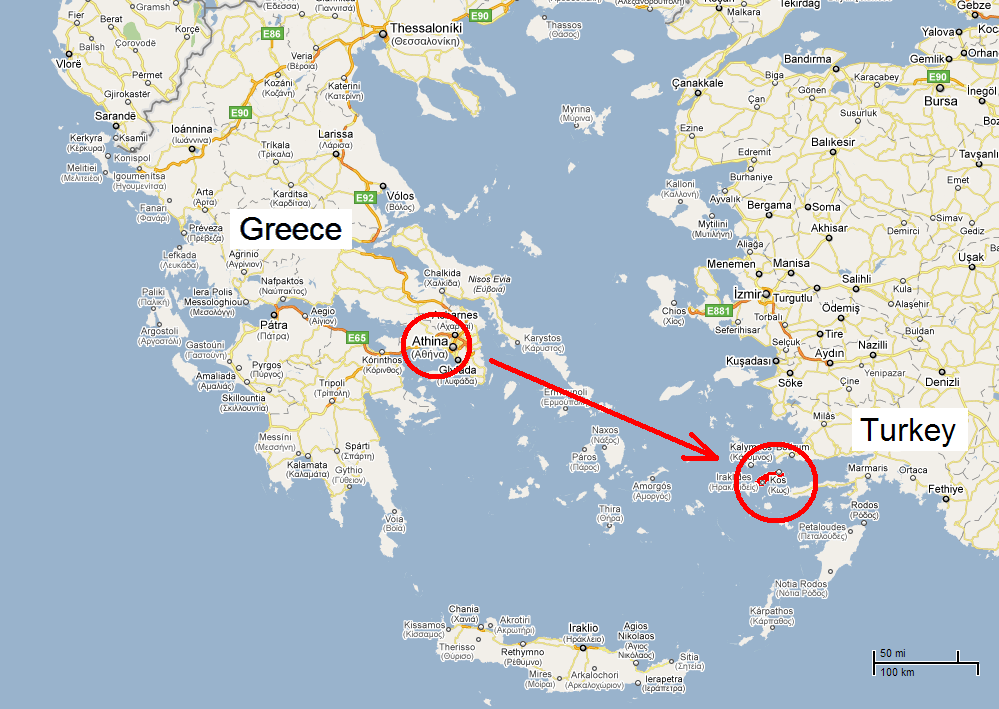
\includegraphics[width=0.8\textwidth]{static/kos-island-map.png}
\end{column}% 
\begin{column}{.38\textwidth}
  		
\includegraphics[width=.30\textwidth]{static/tei-patras-logo.jpg}

  		
\includegraphics[width=.30\textwidth]{static/cardiff_uni_logo.jpg}
\end{column}%
\begin{column}{.38\textwidth}
  		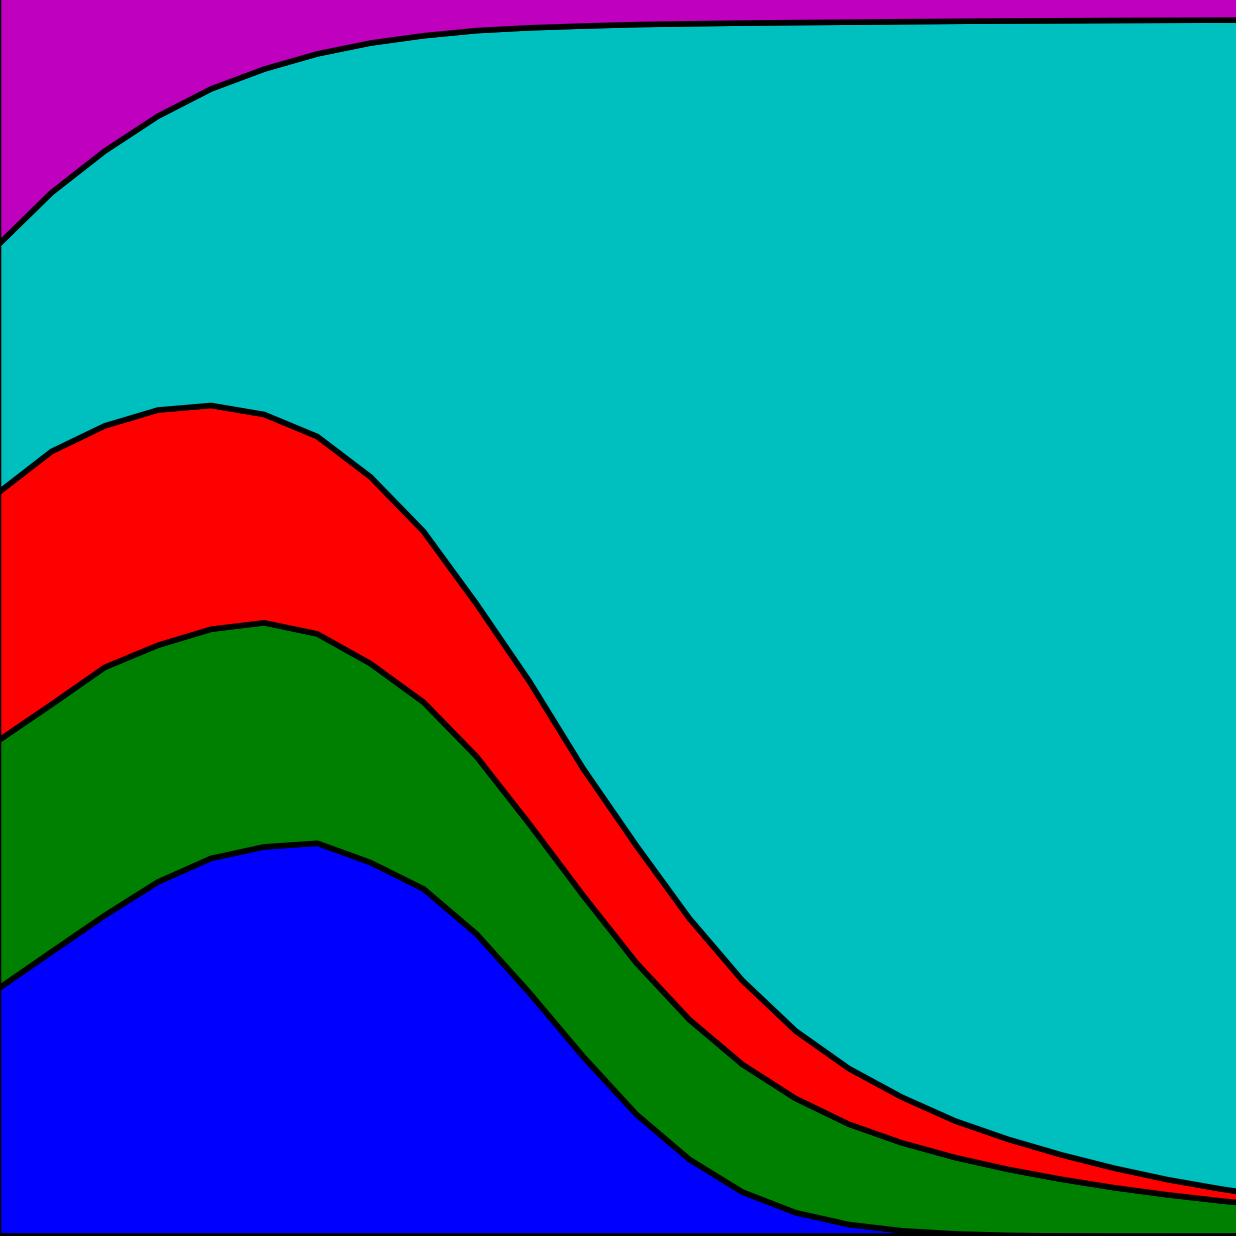
\includegraphics[width=.30\textwidth]{static/axelrod-logo.png}

  		
\includegraphics[width=.30\textwidth]{static/hots_logo.jpg}
\end{column}%
\end{columns}
\end{frame}

\begin{frame}{What I do.}
    \begin{center}
        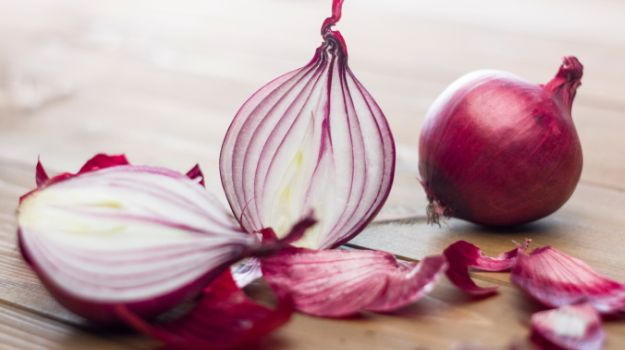
\includegraphics[width=.80\textwidth]{static/onion.jpg}
    \end{center}
\end{frame}

\begin{frame}{What I do.}
    \begin{figure}[htp]
        \centering
            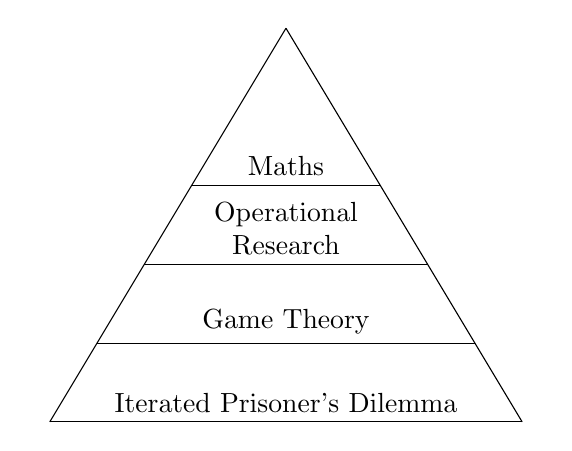
\begin{tikzpicture}
                \coordinate (A) at (-3,0) {};
                \coordinate (B) at ( 3,0) {};
                \coordinate (C) at (0,5) {};
                \draw[name path=AC] (A) -- (C);
                \draw[name path=BC] (B) -- (C);
                \foreach \y/\A in {
                3/Maths,
                2/Operational\\ Research,
                1/Game Theory,
                0/Iterated Prisoner's Dilemma} {
                    \path[name path=horiz] (A|-0,\y) -- (B|-0,\y);
                    \draw[name intersections={of=AC and horiz,by=P},
                          name intersections={of=BC and horiz,by=Q}] (P) -- (Q)
                          node[midway,above,align=center,text width=
                \dimexpr(6em-\y em)*3\relax] {\A};
                }
            \end{tikzpicture}
    \end{figure}
\end{frame}

\begin{frame}{What I do.}
\def\labellist{{" ","(1980)","(1991)","(1992)","(2012)"," ","(2015)"," "}}
    \begin{tikzpicture}
            \begin{axis}[
                height=8cm,
                width=12cm,
                axis lines=left,
                xtick=\empty,
                ytick=\empty,
                nodes near coords={
                                    \pgfmathparse{\labellist[\coordindex]}%
                                    \pgfmathresult }
                ]
    \addplot[color=white,mark=x]
        coordinates{
            (1,1)
            (2,1.1)
            (3,6)
            (4,6.5)
            (5,8.5)
            (6,9)
            (7,9.5)
            (8,12) };
            \end{axis}
    \end{tikzpicture}
\end{frame}

\begin{frame}{My standing in the community.}
    \begin{columns}
        \begin{column}{0.3\textwidth}
            \begin{center}
                
\includegraphics[width=\textwidth]{static/PyDiff.png}
            \end{center}
        \end{column}   
        \begin{column}{0.2\textwidth}
            \begin{center}
                
\includegraphics[width=\textwidth]{static/pyconuk.png}
            \end{center}
        \end{column}
        \begin{column}{0.4\textwidth} 
            \begin{center}
                
\includegraphics[width=\textwidth]{static/or-society-logo.jpg}
            \end{center} 
        \end{column}  
    \end{columns}
\end{frame}

\begin{frame}{My Plans}
	\begin{center}
		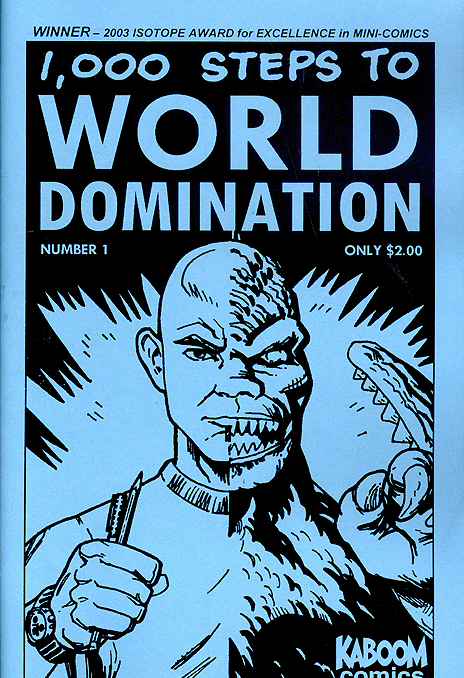
\includegraphics[width=.40\textwidth]{static/evil-mastermind.png}
	\end{center}

\hfill \tiny http://www.sequentialtart.com/reports.php?ID=1971\&issue=2016-08-15

\end{frame}

\begin{frame}{Plans.}
    \begin{center}

        
\includegraphics[height=0.2\textheight]{static/pyconuk.png}
        \hspace{3cm}
        
\includegraphics[height=0.2\textheight]{static/euroscipy.png}
        
        \rule{\textwidth}{2pt}
        \vspace{5pt}

        
\includegraphics[height=0.2\textheight]{static/marc.jpeg}
        \hspace{3cm}
        
\includegraphics[height=0.2\textheight]{static/game-society.png}

        \rule{\textwidth}{2pt}
        \vspace{5pt}

        
\includegraphics[height=0.2\textheight]{static/pycon-namibia.png}


    \end{center}
\end{frame}

\begin{frame}
	\begin{center}
		\huge{\textbf{}}\\~\\
		\small{@NikoletaGlyn}\\
		\small{https://github.com/Nikoleta-v3}\\
		\small{https://github.com/Axelrod-Python/Axelrod}
	\end{center}
\end{frame}

\end{document}